\section{第2章\quad 从低频电路到微波分析}
\begin{frame}
    通常电路分析应用于元件尺寸远小于工作波长、电路中的各元件(如电阻、电容和电感)彼此独立、位置固定的低频电路。这意味着在所讨论的频率范围内,基本电路元件电阻 $R$ 、电容 $C$ 和电感 $L$ 在各自所处的区域内将分别表现为电阻消耗能量、电容存储电能、
    电感产生磁场,低频电路的上述条件使得我们可将低频电路中的所有元件都视为集总元件。而在微波频段这些电路元件不再表现为纯电阻、电容和电感,而是有额外的阻抗和电抗(寄生效应)。在微波频段,同一元件在不同频率下可能会表现出不同的容性、感性或阻性。
\end{frame}

\subsection{基本电路元件}
\begin{frame}{基本电路元件}{电阻$R$}
    \begin{columns}
        \begin{column}{0.3\linewidth}
            \centering
            $I=\frac{V}{R}$
        \end{column}
        \begin{column}{0.7\linewidth}
            \begin{circuitikz}
                \draw (0,0)
                to[V,v=$V$] (0,2)
                to[short] (5,2)
                to[R=$R$] (5,0)
                to[short] (0,0);
                \draw[->] (2,2.2) -- (3,2.2);
                \draw (2.4,2.2) node[anchor=south] {$I$};
            \end{circuitikz}
        \end{column}
    \end{columns}
    \begin{columns}
        \begin{column}{0.5\linewidth}
            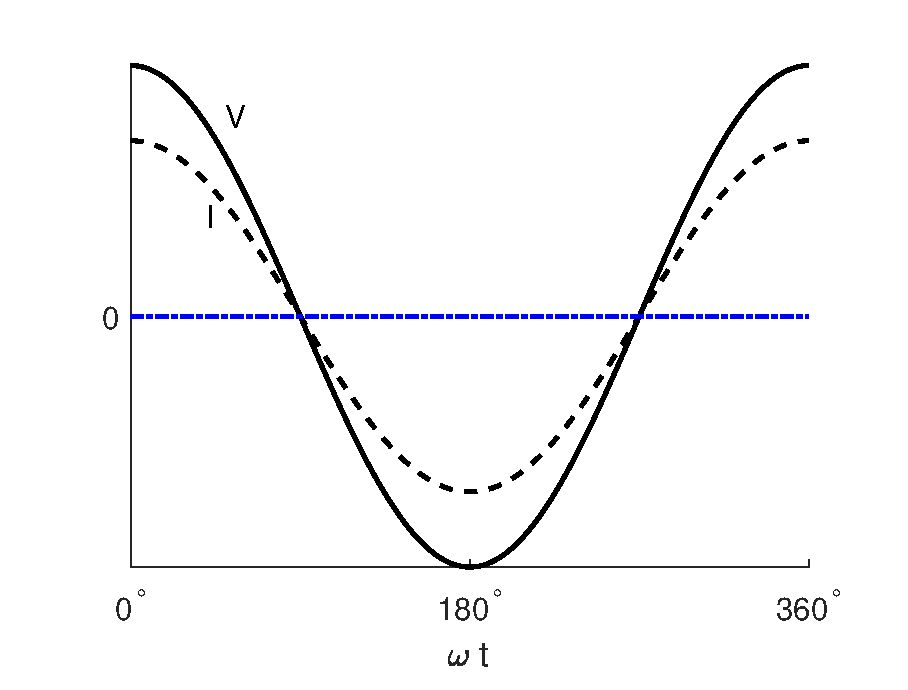
\includegraphics[width=5cm]{Cha2//fig2_1.eps}
        \end{column}
        \begin{column}{0.5\linewidth}
            \tikzset{help lines/.style=thin}
            \tikzset{Karl's grid/.style={help lines,color=blue!50}}
            \begin{tikzpicture}[scale=3]
                \draw (-0.9,0) -- (0.9,0);
                \draw (0,-0.5) -- (0,0.5);
                \draw[red,thick,->] (0,0) -- (0.4,0);
                \draw[blue,thick,->] (0,0) -- (0.7,0);
                \draw (-0.9,0) node[anchor=north] {$180^{\circ}$};
                \draw (0.9,0) node[anchor=north] {$0^{\circ}$};
                \draw (0,-0.5) node[anchor=west] {$270^{\circ}$};
                \draw (0,0.5) node[anchor=west] {$90^{\circ}$};
                \draw (0.4,0) node[anchor=north] {$I$};
                \draw (0.7,0) node[anchor=north] {$V$};
            \end{tikzpicture}
        \end{column}
    \end{columns}
\end{frame}

\begin{frame}{基本电路元件}{电感$L$}
    \begin{columns}
        \begin{column}{0.3\linewidth}
            \begin{align*}
                 & v(t)=L\frac{\mathrm{d} i(t)}{\mathrm{d}t} \quad i(t)=\frac{1}{L}\int_0^t v(t)\mathrm{d}t \\
                 & v(t)=V_0\cos \omega t                                                                    \\
                 & I = \frac{1}{L}\int V_0\cos\omega t \mathrm{d}t=\frac{V_0\sin\omega t}{\omega L}
            \end{align*}
        \end{column}
        \begin{column}{0.7\linewidth}
            \begin{circuitikz}
                \draw (0,0)
                to[V,v=$V$] (0,2)
                to[short] (5,2)
                to[L=$L$] (5,0)
                to[short] (0,0);
                \draw[->] (2,2.2) -- (3,2.2);
                \draw (2.4,2.2) node[anchor=south] {$I$};
            \end{circuitikz}
        \end{column}
    \end{columns}
    \begin{columns}
        \begin{column}{0.5\linewidth}
            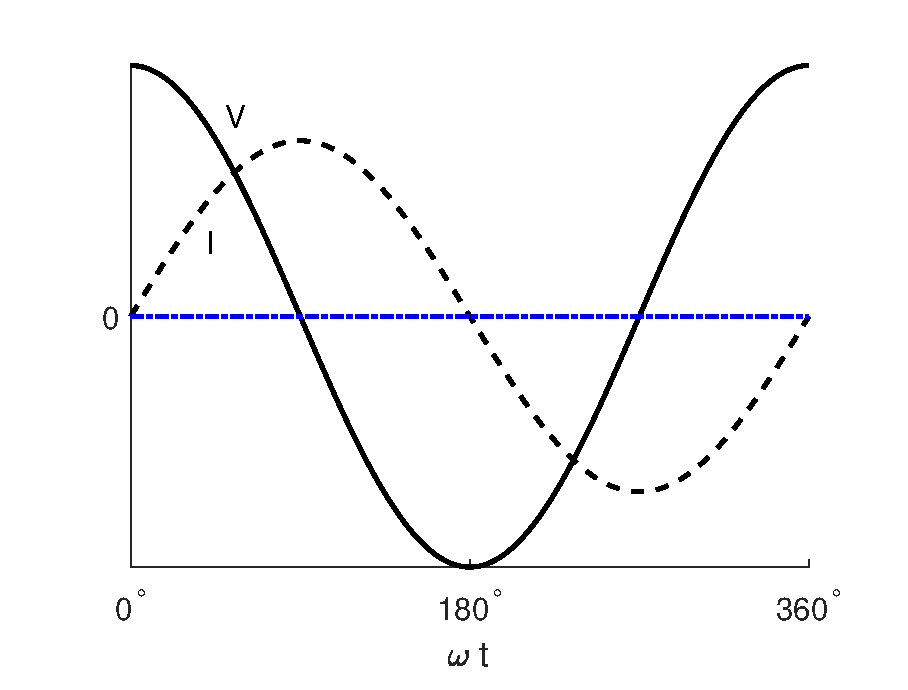
\includegraphics[width=5cm]{Cha2//fig2_2.eps}
        \end{column}
        \begin{column}{0.5\linewidth}
            \tikzset{help lines/.style=thin}
            \tikzset{Karl's grid/.style={help lines,color=blue!50}}
            \begin{tikzpicture}[scale=3]
                \draw (-0.9,0) -- (0.9,0);
                \draw (0,-0.5) -- (0,0.5);
                \draw[red,thick,->] (0,0) -- (0,-0.4);
                \draw[blue,thick,->] (0,0) -- (0.7,0);
                \draw (-0.9,0) node[anchor=north] {$180^{\circ}$};
                \draw (0.9,0) node[anchor=north] {$0^{\circ}$};
                \draw (0,-0.5) node[anchor=west] {$270^{\circ}$};
                \draw (0,0.5) node[anchor=west] {$90^{\circ}$};
                \draw (0,-0.4) node[anchor=west] {$I$};
                \draw (0.7,0) node[anchor=north] {$V$};
            \end{tikzpicture}
        \end{column}
    \end{columns}
\end{frame}

%\begin{comment}
\begin{frame}{基本电路元件}{电容$C$}
    \begin{columns}
        \begin{column}{0.3\linewidth}
            \begin{align*}
                 & i(t)=C \frac{\partial v(t)}{\partial t} \quad v(t)=\frac{1}{C}\int_0^t i(t)\mathrm{d}t \\
                 & v(t)=V_0\cos \omega t                                                                    \\
                 & I = C \frac{\partial v(t)}{\partial t}=-V_0\omega C\sin\omega t
            \end{align*}
        \end{column}
        \begin{column}{0.7\linewidth}
            \begin{circuitikz}
                \draw (0,0)
                to[V,v=$V$] (0,2)
                to[short] (5,2)
                to[C=$C$] (5,0)
                to[short] (0,0);
                \draw[->] (2,2.2) -- (3,2.2);
                \draw (2.4,2.2) node[anchor=south] {$I$};
            \end{circuitikz}
        \end{column}
    \end{columns}
    \begin{columns}
        \begin{column}{0.5\linewidth}
            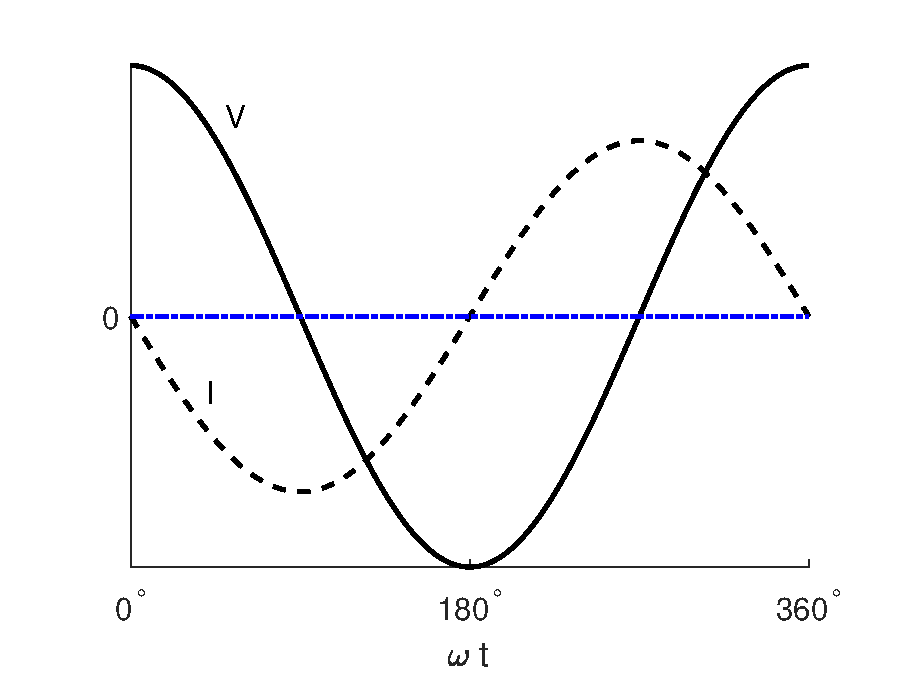
\includegraphics[width=5cm]{Cha2//fig2_3.eps}
        \end{column}
        \begin{column}{0.5\linewidth}
            \tikzset{help lines/.style=thin}
            \tikzset{Karl's grid/.style={help lines,color=blue!50}}
            \begin{tikzpicture}[scale=3]
                \draw (-0.9,0) -- (0.9,0);
                \draw (0,-0.5) -- (0,0.5);
                \draw[red,thick,->] (0,0) -- (0,0.4);
                \draw[blue,thick,->] (0,0) -- (0.7,0);
                \draw (-0.9,0) node[anchor=north] {$180^{\circ}$};
                \draw (0.9,0) node[anchor=north] {$0^{\circ}$};
                \draw (0,-0.5) node[anchor=west] {$270^{\circ}$};
                \draw (0,0.5) node[anchor=west] {$90^{\circ}$};
                \draw (0,0.4) node[anchor=west] {$I$};
                \draw (0.7,0) node[anchor=north] {$V$};
            \end{tikzpicture}
        \end{column}
    \end{columns}
\end{frame}
%\end{comment}

\subsection{电压和电流相量}
\begin{frame}{电压和电流相量}
    相量电压 $V$ 来表示正弦电压 $v(t)$ ; 相量电流 $I$ 来表示产生的电流 $i(t)$
    \begin{align*}
         & v(t)=\mathrm{Re}[V\mathrm{e}^{\mathrm{j}\omega t}] \\
         & i(t)=\mathrm{Re}[I\mathrm{e}^{\mathrm{j}\omega t}]
    \end{align*}
    $L$ 和 $C$ 元件的电抗是单位为 $\Omega$ 的正实数
    $$X_L = \omega L(\Omega) \quad X_C = \frac{1}{\omega C}(\Omega)$$
    阻抗
    \begin{align*}
        & Z_L=\mathrm{j} \omega L \quad Z_C=-\mathrm{j} \frac{1}{\omega C} \\
        & Z=R+\mathrm{j} (X_L-X_C)=R+\mathrm{j} (\omega L-1/\omega C)
   \end{align*}
\end{frame}

\subsection{阻抗和导纳}
\begin{frame}{阻抗和导纳}
$$X_L=\omega L, \omega=2\pi f$$
频率为$1GHz$,一个 $1nH$ 的电感电抗值为$6.28\Omega$,这样,在其他频率下的其他电感的电抗值为
$$X_L=6.28fL\text{(f的单位GHz,L的单位nH)}$$
同理
$$X_C=\frac{1}{\omega C}, \omega=2\pi f$$
频率为$1GHz$,一个 $1pF$ 的电容电抗值为$159\Omega$,这样,在其他频率下的其他电容的电抗值为
$$X_C=159/fC\text{(f的单位GHz,C的单位pF)}$$
串联阻抗相加
\begin{align*}
    &Z_1=a+\mathrm{j} b \quad Z_2=c+\mathrm{j} d\\
    &Z_T=Z_1+Z_2=(a+c)+\mathrm{j} (b+d)
\end{align*}
\end{frame}

\begin{frame}{阻抗和导纳}
    $$B_L=\frac{1}{X_L}=\frac{1}{\omega L}$$
    电感的导纳为
    $$-\mathrm{j} B_L=\frac{1}{\mathrm{j} X_L}=\frac{1}{\mathrm{j} \omega L}=\frac{-\mathrm{j} }{\omega L}$$
    同理
    $$B_C=\frac{1}{X_C}=\frac{1}{1/\omega C}=\omega C$$
    电容的导纳为
    $$\mathrm{j} B_C=\frac{1}{-\mathrm{j} X_C}=\frac{1}{-\mathrm{j} /\omega C}=\mathrm{j} \omega C$$
    并联导纳相加
    \begin{align*}
        &Z_T=\frac{1}{Y_T}=\frac{1}{Y_1+Y_2}
    \end{align*}
    \end{frame}

\subsection{电路分析基本定律}
\begin{frame}{电路分析基本定律}
    \begin{columns}
        \begin{column}{0.5\linewidth}
            \centering
            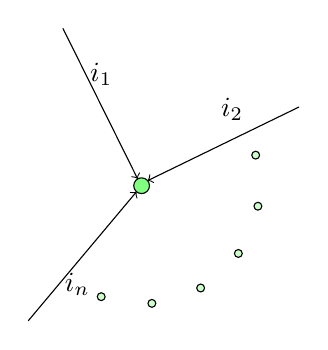
\begin{tikzpicture}
                \filldraw[fill=green!50!white] (0,0) circle [radius=1mm];
                \draw[->] (2cm,1cm) -- ({1mm*cos(40)},{1mm*sin(40)});
                \draw ({1.5cm*cos(40)},{1.5cm*sin(40)}) node {$i_2$};
                \draw[->] (-1cm,2cm) -- ({1mm*cos(120)},{1mm*sin(120)});
                \draw ({1.5cm*cos(110)},{1.5cm*sin(110)}) node {$i_1$};
                \draw[->] ({2.24cm*cos(230)},{2.24cm*sin(230)}) -- ({1mm*cos(230)},{1mm*sin(230)});
                \draw ({1.5cm*cos(237)},{1.5cm*sin(237)}) node {$i_n$};

                \foreach \x in {250,275,300,325,350,15}
                \filldraw[fill=green!20!white] ({1.5cm*cos(\x)},{1.5cm*sin(\x)}) circle [radius=0.5mm];
            \end{tikzpicture}
        \end{column}
        \begin{column}{0.5\linewidth}
            \centering
            $$\sum_{n=1}^N i_n(t)=0$$
        \end{column}
    \end{columns}

    \begin{columns}
        \begin{column}{0.8\linewidth}
            \begin{circuitikz}
                \centering
                \draw (0,0) to[R,o-o] (0,3)
                to[short,o-o] (2,3)
                to[R] (5,3)
                to[short,-o] (6,3)
                to[R,-o] (6,0);
                \draw[dashed] (6,0) to[short,o-o] (4,0);
                \draw (4,0) to[R,o-] (1,0);
                \draw[dashed] (1,0) to[short,-o] (0,0);
                \draw[dashed] (2,3) to[short] (2,1.5);
                \draw (4,0) to[short] (4,1.5);
                \draw[dashed] (4,1.5) to[short] (4,2.5);
                
                \draw (6,3) -- (6.5,3);
                \draw[dashed] (6.5,3) -- (8,3);
                \draw (6,0) -- (6.5,0);
                \draw[dashed] (6.5,0) -- (8,0);
                \draw (0,3) -- (-0.5,3);
                \draw[dashed] (-0.5,3) -- (-2,3);
                \draw (0,0) -- (-0.5,0);
                \draw[dashed] (-0.5,0) -- (-2,0);

                \draw(-0.5,2.5) node[anchor=east] {+};
                \draw(-0.5,0.5) node[anchor=east] {-};
                \draw(-0.5,1.5) node[anchor=east] {$v_M$};

                \draw(6.5,2.5) node[anchor=west] {+};
                \draw(6.5,0.5) node[anchor=west] {-};
                \draw(6.5,1.5) node[anchor=west] {$v_2$};

                \draw(2.5,3.2) node[anchor=south] {+};
                \draw(4.5,3.2) node[anchor=south] {-};
                \draw(3.5,3.2) node[anchor=south] {$v_1$};

                \draw(1.5,0.2) node[anchor=south] {-};
                \draw(3.5,0.2) node[anchor=south] {+};
                \draw(2.5,0.2) node[anchor=south] {$v_m$};
            \end{circuitikz}
        \end{column}
        \begin{column}{0.2\linewidth}
            \centering
            $$\sum_{m=1}^M v_m(t)=0$$
        \end{column}
    \end{columns}
\end{frame}

\begin{frame}{电路分析基本定律}
    \centering
    \begin{tabular}{ccc}
        \toprule
         名称 & 时域                                 & 频域                      \\
        \midrule
         电容 & $i(t)=C\mathrm{d}v(t)/\mathrm{d}t$   & $I=\mathrm{j}\omega CV$ \\
         电感 & $v(t)=L\mathrm{d}i(t)/\mathrm{d}t$   & $V=\mathrm{j}\omega LI$ \\
         欧姆定律 & $v(t)=Ri(t)$                     & $V=RI$                   \\
         广义欧姆定律 & $v(t)=Ri+\frac{1}{C} \int_0^t i\mathrm{d}t+L\mathrm{d}i/\mathrm{d}t$ & \makecell{$V(\omega)=Z(\omega)I(\omega)$ \\ $Z=R+\mathrm{j}(\omega L-1/\omega C)$} \\ % 表格内换行
         KCL & $\sum\limits_{n=1}^N i_n(t)=0$       & $\sum\limits_{n=1}^N I_n(\omega)=0$ \\
         KVL & $\sum\limits_{m=1}^M v_m(t)=0$       & $\sum\limits_{m=1}^M V_m(\omega)=0$ \\
        \bottomrule
    \end{tabular}
\end{frame}

\subsection{正弦稳态条件下的功率计算}
\begin{frame}{正弦稳态条件下的功率计算}
    \centering
    \tikzset{
        rect1/.style = {
                shape = rectangle, % 指定样式
                minimum height = 2cm,
                minimum width = 3cm,
                align = center, % 文字居中
            }
    }
    \begin{tikzpicture}
        \node (a) [rect1,draw=black,text width=2cm] {源或信号发生器};
        \node[right of=a,xshift=100pt] (b) [rect1,draw=black,text width=2cm] {线性负载网络$N$};
        \draw (1.5cm,0.5cm) -- (2.2cm,0.5cm);
        \draw (2.3cm,0.5cm) -- (3cm,0.5cm);
        \draw (1.5cm,-0.5cm) -- (2.2cm,-0.5cm);
        \draw (2.3cm,-0.5cm) -- (3cm,-0.5cm);
        \draw (2.25cm,0.5cm) circle [radius=0.5mm];
        \draw (2.25cm,-0.5cm) circle [radius=0.5mm];
        \draw[->] (2cm,-1cm) -- (2cm,-0.1cm) -- (2.4cm,-0.1cm);
        \draw (2cm,-1cm) node[anchor=north] {$Z,Y$};
        \draw[->] (2.4cm,0.75cm) -- (2.8cm,0.75cm);
        \draw (2.4cm,0.75cm) node[anchor=south] {$i(t)$};
        \draw (2.25cm,0.6cm) node[anchor=north] {$+$};
        \draw (2.25cm,-0.63cm) node[anchor=south] {$-$};
    \end{tikzpicture}\\
    \begin{columns}
        \begin{column}{0.5\linewidth}
            \centering
            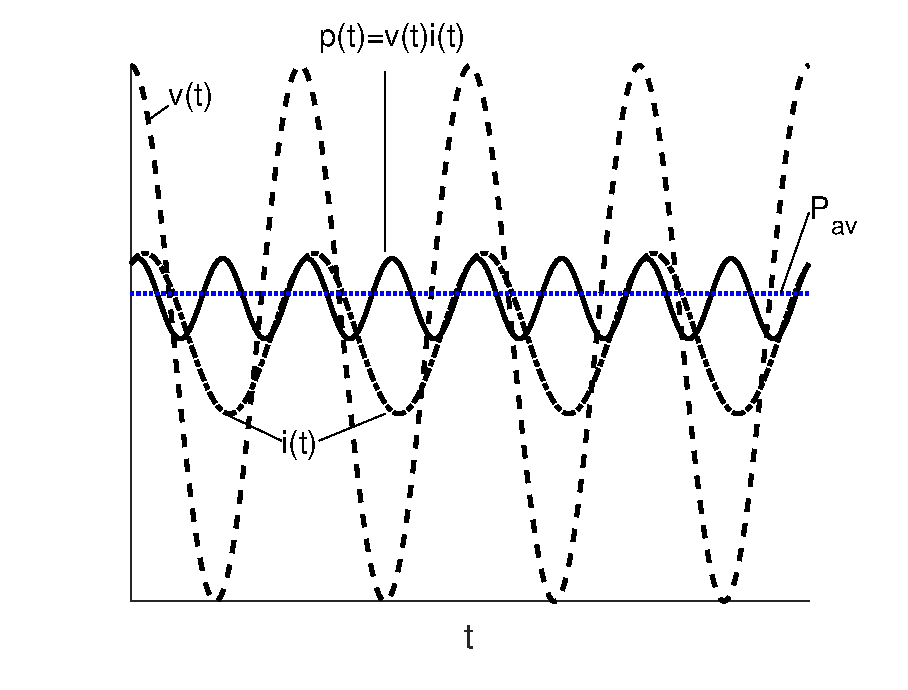
\includegraphics[width=5cm]{Cha2//fig2_8.eps}
        \end{column}
        \begin{column}{0.5\linewidth}
            瞬时功率:$p(t)=v(t)i(t)$ \\
            平均功率:$P_{av}=\dfrac{1}{T}{\displaystyle \int_0^T}p(t)\mathrm{d}t=\dfrac{1}{T}{\displaystyle \int_0^T}v(t)i(t)\mathrm{d}t$\\
            复功率:$P=\dfrac{1}{2}VI^*$
        \end{column}
    \end{columns}
\end{frame}

\subsection{分贝}
\begin{frame}{分贝}
\begin{align*}
    &N(\mathrm{dB})=10\lg(P_2/P_1)\\
    &\text{分贝瓦}(\mathrm{dBW}):N(\mathrm{dBW})=10\lg(P_2/1\mathrm{W})\\
    &\text{分贝毫瓦}(\mathrm{dBmW}):N(\mathrm{dBmW})=10\lg(P_2/1\mathrm{mW})\\
    &\text{分贝微瓦}(\mathrm{dB\mu W}):N(\mathrm{dB\mu W})=10\lg(P_2/1\mathrm{\mu W})
\end{align*}
奈培$(Np)$:奈培定义为两个电流、电压或场强的比值的自然对数(以$e$为底的对数),它是表征衰减的单位。如果电压从$V_1$衰减至$V_2$,则有\\
\begin{align*}
    &V_2/V_1=e^{-N}\\
    &N(\mathrm{Np})=\ln(V_2/V_1)^{-1}=-\ln(V_2/V_1)\\
    &1\mathrm{Np}=-\ln(V_2/V_1)\Rightarrow V_2/V_1=1/\mathrm{e}\\
    &1\mathrm{Np}=20\lg[1/(V_2/V_1)]=20\lg\mathrm{e}=8.686\mathrm{dB}
\end{align*}
\end{frame}

\subsection{趋肤效应}
\begin{frame}{趋肤效应}
    \begin{columns}
        \begin{column}{0.6\linewidth}
            \centering
            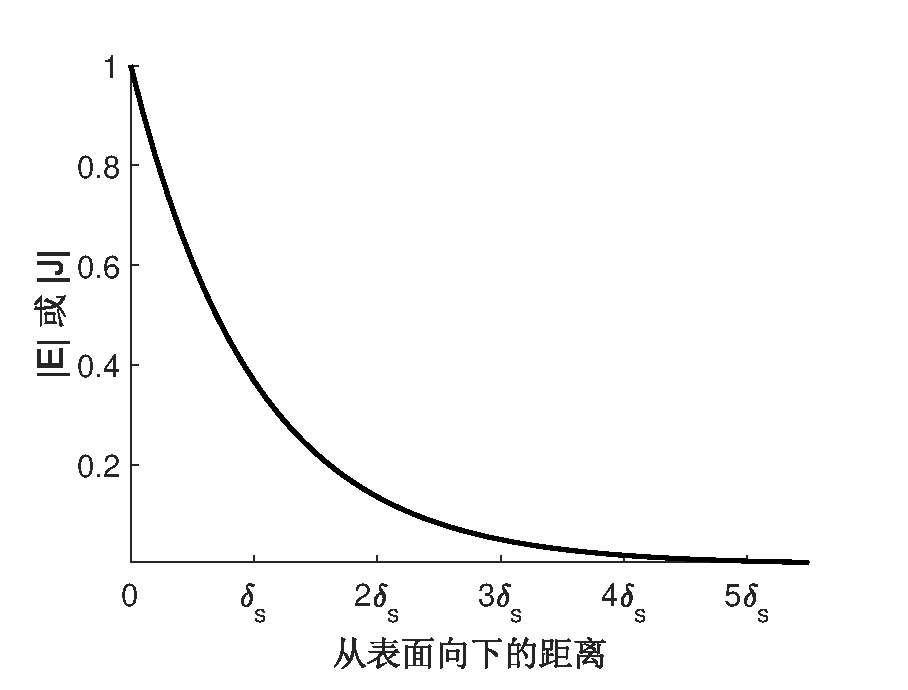
\includegraphics[width=6cm]{Cha2//fig2_9.eps}
        \end{column}
        \begin{column}{0.4\linewidth}
            \centering
            \begin{align*}
                &\vec J = \sigma \vec E\\
                &\vec J = \vec J_0 \mathrm{e}^{-z/\delta_s}\\
                &\delta_s = \frac{1}{\sqrt{\pi f\mu\sigma}}\\
                & R_{AC} = \frac{1}{\pi D\delta_S\sigma} \\
                & R_{DC} = \frac{1}{\pi(D^2/4)\sigma}
            \end{align*}
        \end{column}
    \end{columns}

\end{frame}